\chapter{Litterature}

This chapter presents different concepts used in this project. Images are introduced, then concepts of edge detection and noise removal are explained, allonw with a cellular automata algorithm and the \gls{CLAP} algorithm. Finally the Freeman chain codes are described, as well as some features that can be extracted from it. 

\section{Images}

An image is represented by a width, an heigth, colors (stocked in pixel values, i.e. positive integers), and a color model. A color model describes how the colors are represented, that is how many values should be used in order to represent a color \cite{bib:image:ColorModel}. Multiples color models exist, for example : 
\begin{itemize}
	\item RGB, where a color is represented by the three primary colors (red, green and blue)
	\item CMY, where a color is represented by a combinaison of cyan, magenta and yellow colors
\end{itemize}

% cours de jpeg 

~~

%\begin{figure}[h]
\begin{wrapfigure}{R}{0.3\textwidth}
	\centering
	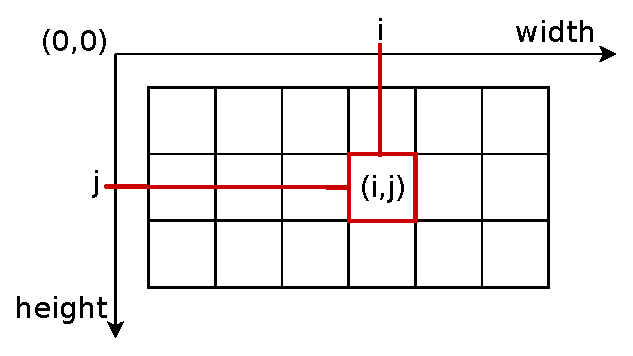
\includegraphics[width=0.3\textwidth]{images/axis/axis_representation}
	\caption{Axis representation}
	\label{fig:axis representation}
%\end{figure}
\end{wrapfigure}


This project is dealing with three types of images : RGB, Grey and Monochromatic images. A grey image is an image where the pixels are represented in a grey scale by only one value, the grey value (which can have any integer values between 0 and 255 included). In other words, there is 256 possible colors in a grey images, which are all shade of grey. In a monochromatic image, only two colors are represented, black (with the value 0) and white (with the value 255). The axis we used to represent an image are illustrated on the \vref{fig:axis representation}. 

%Once an image is loaded in the RGB color model, we converted it into a grey image in order to reduce the number of information present in the image and lower the complexity. The monochromatic image were used in order to determinate edges and extract the objects in the image.

~~

The grey value of a RGB pixel is determined by doing the average of the red, green and blue values. As for the monochromatic image, first a threshold value is defined, then a pixel is represented in black if it's grey value is strictly under the threshold, and in white otherwise (the equation \ref{eq:threshold} show it in a more mathematical point of view) \cite{bib:image:Threshold}.

\begin{equation} \label{eq:threshold}
mono_{threshold}(greyValue) = 
	\begin{cases}
		BLACK & \text{if } greyValue < threshold \\
		WHITE & \text{otherwise} \\ 
	\end{cases}
\end{equation}







\section{Edge detection}

Edge detection regroups differents mathematical methods, where the goal is to identify the change of brightness in the images. An edge is defined as the segments points in where the brightness changes \cite{bib:filter:wikipedia}. Three edge detection methods will be presented in this section : the Sobel, the Laplacian and the Canny operators. These operations detect edges by applying a convolution between an image and a certain mask. The differents masks are given in the \vref{tab:edge detection:masks}.

\begin{table}[ht]	
	\begin{subtable}[b]{0.2\textwidth}
		\centering
		\begin{tabular}{|c|c|c|}
			\hline 
			-1 & 0 & 1 \\ \hline
			-2 & 0 & 2 \\ \hline
			-1 & 0 & 1 \\ \hline
		\end{tabular}
		\caption{Sobel, X axis}
		\label{tab:edge detection:sobel:x}
	\end{subtable}% 
	\begin{subtable}[b]{0.2\textwidth}
		\centering
		\begin{tabular}{|c|c|c|}
			\hline 
			-1 & -2 & -1 \\ \hline
			0 & 0 & 0 \\ \hline
			1 & 2 & 1 \\ \hline
		\end{tabular}
		\caption{Sobel, Y axis}
		\label{tab:edge detection:sobel:y}	
	\end{subtable}%
	\begin{subtable}[b]{0.2\textwidth}
		\centering
		\begin{tabular}{|c|c|c|}
			\hline 
			-1 & -1 & -1 \\ \hline
			-1 & 8  & 0 \\ \hline
			-1 & -1 & -1 \\ \hline
		\end{tabular}
		\caption{Laplacian filter}
		\label{tab:edge detection:laplacian}
	\end{subtable}% 
	\begin{subtable}[b]{0.2\textwidth}
		\centering
		\begin{tabular}{|c|c|c|}
			\hline
			-1 & 0 & 1 \\ \hline
		\end{tabular}
		\caption{Canny, X axis}
		\label{tab:edge detection:canny:x}
	\end{subtable}%
	\begin{subtable}[b]{0.2\textwidth}
		\centering
		\begin{tabular}{|c|}
			\hline
			-1 \\ \hline
			0 \\ \hline
			1 \\ \hline
		\end{tabular}
		\caption{Canny, Y axis}
		\label{tab:edge detection:canny:y}
	\end{subtable}
	
	\centering 
	\caption{Edge detection masks}
	\label{tab:edge detection:masks}
\end{table}

% présentation des 3 filtres 

%The Sobel operator can be obtain by using a convolution between each pixel of the images and the 

~~ 

The Sobel operator calculates the gradiant of each pixel on the image. It is done by applying a convolution on the image with the two masks given on \vref{tab:edge detection:sobel:x,tab:edge detection:sobel:y}, which are filters that estimates the gradiant in the horizontal and vertical direction  \cite{bib:filter:sobelRuby}. $G_x$ will be the result of the convolution between the image and the $x$ axis filter (same for $G_y$ but with the $y$ axis filter). The gradiant of the resulting image can then be obtain by applying the \vref{eq:edge detection:gradiant}. The Canny operator works in the same way as the Sobel operator. Moreover, the \vref{eq:edge detection:gradiant} can be simplified as the \vref{eq:edge detection:gradiant:simplified} using the manhattan distance \cite{bib:filter:canny}. The first equation will be used for sobel, and the second for canny. 

% The gradient of the image is calculated for each pixel position in the image. 

\noindent\begin{tabularx}{\textwidth}{@{}XX@{}}
	\begin{equation} \label{eq:edge detection:gradiant}
		|G| = \sqrt{G_{x}^2 + G_{y}^2}
	\end{equation} & 
	\begin{equation} \label{eq:edge detection:gradiant:simplified}
		G = |G_x| + |G_y|
	\end{equation}
\end{tabularx}





\noindent\begin{minipage}{0.55\textwidth}


\section{Noise removal}


Noise removal, or noise reduction, is the process of removing noise from a signal, like an image. Noise can be introduced in an image during the capture of that image, which mean that some pixels don't have the right values \cite{bib:noise:wikipedia}. Multiple techniques exist in order to remove this noise, like the gaussian blur or the weighted average filter. For example, the median filter is one of them, where the new value of each pixel will be the median value of the pixel neighborhood (in 8-connexity) \cite{bib:noise:ImageFiltering}.


\section{Cellular Automata algorithm}

The algorithms presented in the paper \cite{bib:filter:CA} are image noise reduction algorithms based on cellular automata. For this project, it has been decided to implement the second version of the algorithm. A cellular automaton concists of a large number of simple individuals, called cells, which have a state (e.g. "on" and "off"). During one iteration, each cell updates its state depending on its own state and on the state of the neighbor cells. Two types od neighborhooh exists : the 4-connexity (Von Neumann) and the 8-connexity (Moore) neighborhood. For this algorithm, it is the Moor neighborhood that is used. In the case of the second algorithm, each pixel will be updated by taking the average value of his 8-connexity neighborhood (him included), except the minimum and the maximum values. The \vref{fig:diagram:flowchart:CAII} explains the procedure with a flowchart.


\end{minipage} \hfill 
\begin{minipage}{0.4\textwidth}

%%%%%%%%%%%%%%%%%%%%%%%%%%%%%%%%%%%%%%%%%%%%%%%%%%%%%%
%\begin{wrapfigure}{R}{0.4\textwidth}
\begin{figure}[H]
	\centering
	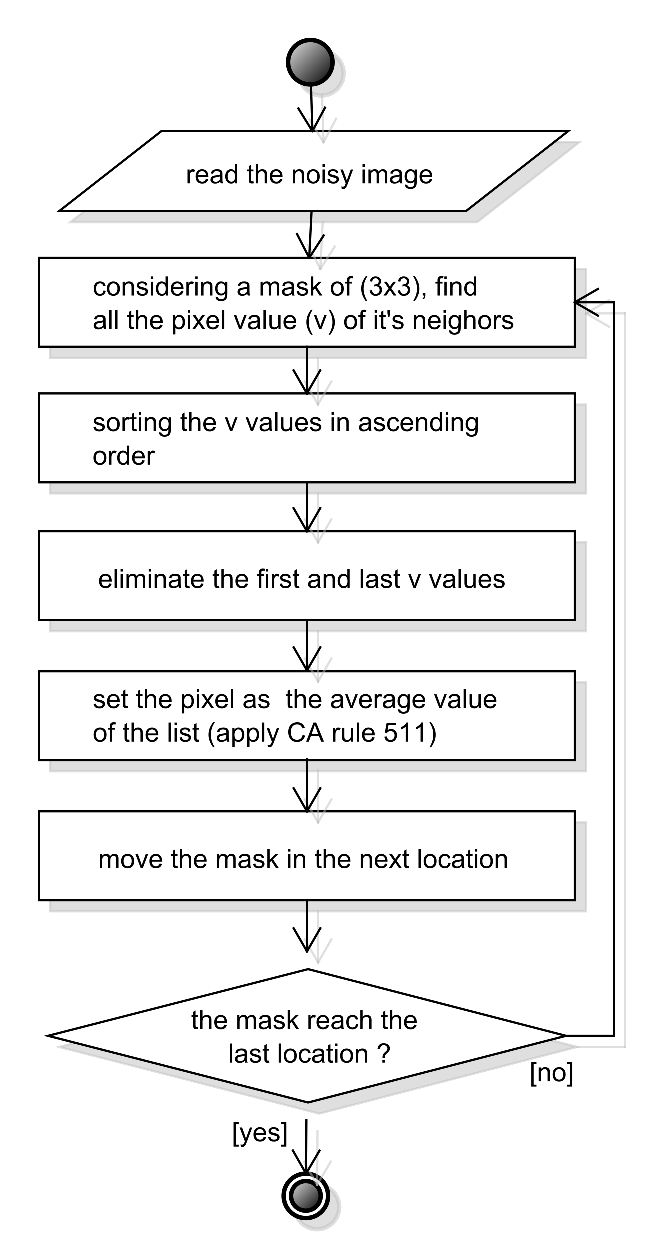
\includegraphics[width=\textwidth]{images/diagrams/flowchart_CAII}
	\caption{CA II flowchart \cite{bib:filter:CA}}
	\label{fig:diagram:flowchart:CAII}
\end{figure}
%\end{wrapfigure}

\end{minipage}

\newpage 


\section[CLAP]{Cellular Logic Array Processing algorithm}

The \acrfull{CLAP} \gls{algorithm} is a new algorithm for extracting volumetric edges from 3D images. Volumetric edges refers to lines, curves and points represented in a 3D digital space. \gls{CLAP} combines notions of Markov's normal algorithms and Von Neuman's cellular automata. A threshold value is required. The principe is the following : for each pixel, the minimal and the maximal pixel values are determinated from the 4-connexity pixel neighborhood (including the actual pixel). Then, the difference between the maximum and the minimum is calculated. If that difference is inferior or equal to the given  threshold value, all the 4-connexity pixel neighbors are set to 0. Pixel values are not changes if it's not the case \cite{bib:filter:EdgeWithCLAP}. The \gls{algorithm} as given in the paper is shown at the \vref{sec:annexe:clap}. 







\section{Freeman Chain Code}

% A feature is defined as something in the image that have a certain shape and edges.  


The Freeman Chain Code is a coding edge algorithm. It allows to represent a shape given in a bimary image (monochromatic) by it's edge. It's first purpose is to compress the data, as we pass from a binary image to a chain (or list) of code representing the shape of the edge \cite{bib:chain:ParametreGeometriqueChaineFreeman}. In other words, it's a data structure for representing the boundary of a feature \cite{bib:chain:DigitalImageProcessing}.

~~ 

In order to extract the chain code of a shape in a binary image, it is necessary to start from on of the end edges. For this project, it has been decided to start from the most left upper edge point of the shape, i.e. there isn't any other edge point that is at the left of the starting point. In order to have this starting point, the image has been travelled from up to down, and then from left to right, as it is shown on the \vref{fig:chain code:course order}.


~~


Once the starting point is determined, it is then possible to follow the boundary in the anticlockwise direction. Then, depending on the direction, a code is generated according to the following direction scheme illustrated with the \vref{fig:chain code:direction scheme star}, where the central point of the star represent the current boundary pixel. For example, if the next boundary pixel is on the top of the current one, the code 2 will be generated. 


\begin{figure}[H]
	\centering
	
  	\begin{subfigure}[b]{0.5\textwidth}
    	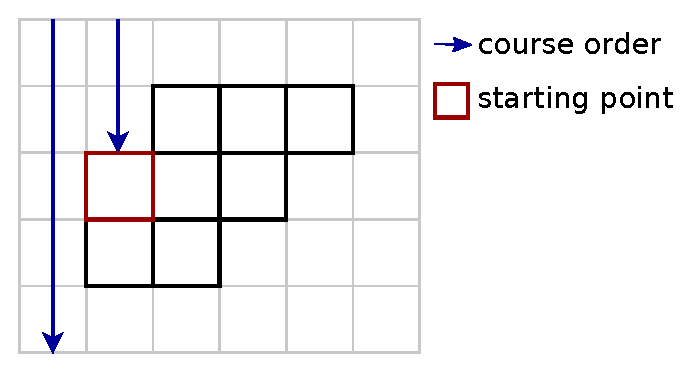
\includegraphics[width=\textwidth]{images/chain_code/course_order}
		\caption{Course order of the binary image \cite{bib:chain:ParametreGeometriqueChaineFreeman}}
		\label{fig:chain code:course order}	
  	\end{subfigure}
  	\begin{subfigure}[b]{0.4\textwidth}
  		\centering
    	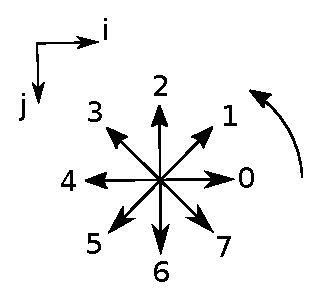
\includegraphics[width=0.5\textwidth]{images/chain_code/direction_scheme_star}
    	\caption{Direction scheme star \cite{bib:chain:ParametreGeometriqueChaineFreeman}}
		\label{fig:chain code:direction scheme star}
  	\end{subfigure}
	
	\caption{Course order and direction scheme star}
\end{figure}




Moreover, in order to support more complexe shapes, the pixel neibors of the current boundary pixel are travelled depending on the last generated code (i.e. on the last direction). In other words, the stating point of the star is changed depending on the last direction. The first pixel neibor that should be visited must be the previous pixel boundary (i.e. the origin of the direction used to get on the current pixel). For example, the chain code "6011445" can be produced with the shape given on the \vref{fig:chain code:course order}. The \vref{fig:chain code:example} explains the procedure. 

\begin{figure}[H]
	\centering
	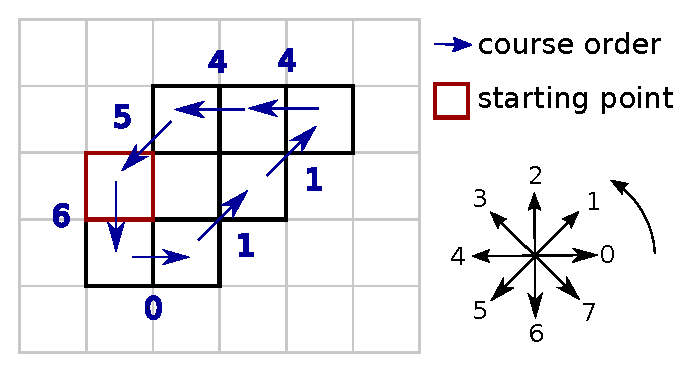
\includegraphics[width=0.5\textwidth]{images/chain_code/example}
	\caption{Example of a chain code}
	\label{fig:chain code:example}	
\end{figure}

~~

Chain codes are translation invariant but depend on rotation, which mean that differents chain codes will be produced for the shape and it's rotation. It is possible to make the chain code invariant to rotation by using the fisrt difference of the chain code instead, i.e. each code will be substracted with the previous code modulo 8 (as we are in 8-connexity). The new chain will be named differential chain code \cite{bib:chain:RepresentationAndDescription}. The calculation of the differential chain code of the shape of the \vref{fig:chain code:course order} is given with the \vref{tab:chain code:differential chain code}.
\begin{equation} \label{eq:chain code:differential chain code}
d_i = code_i - code_{(i-1) \bmod N} \bmod 8
\end{equation}

%%%%%%%%%%%%%%%%%%%%%%%%%%%%%%%%%%%%%%%
\begin{comment}
	\begin{cases}
		code_i - code_{i-1} mod 8 & \text{if } i \not = 1 \\
		code_i - code_{N} mod 8 & \text{otherwise} \\
	\end{cases}
\end{comment}
%%%%%%%%%%%%%%%%%%%%%%%%%%%%%%%%%%%%%%%


\begin{table}[ht]
	\centering
	\caption{Example of a differential chain code}
	\label{tab:chain code:differential chain code}
	\begin{tabular}{rccccccc}
\toprule 
chain code   & 6     & 0     & 1     & 1     & 4     & 4     & 5     \\
substraction & 6 - 5 & 0 - 6 & 1 - 0 & 1 - 1 & 4 - 1 & 4 - 4 & 5 - 4 \\
value     	 & 1     & -6    & 1     & 0     & 3     & 0     & 1     \\
modulo 8 (differential code)  	 & 1     & 2     & 1     & 0     & 3     & 0     & 1     \\ 
\bottomrule 
	\end{tabular}
\end{table}


% http://poseidon.csd.auth.gr/LAB_PUBLICATIONS/Books/dip_material/chapter_7/chap7en.pdf 
% http://www.ece.uvic.ca/~aalbu/computer%20vision%202009/Lecture%2022.%20Shape%20description-contours.pdf 
% http://www.vis.uky.edu/~ryang/teaching/cs635-2016spring/Lectures/16-representation.pdf 




\section{Feature extraction from a chain code}

After extracting the chain code from a shape, it is then possible to extracts features from it. A feature is another piece of information or characteristic which is relevent for solving a task \cite{bib:extraction:definition}. The following features were extracted : 
\begin{itemize}
	\item the perimeter (the number of boundary pixels), the width and the height
	\item the area, which is the number of pixels in the region or shape 
	\item the compactness 
	\item the circularity 
	\item the curvature, representing the successive changes in directions 
	\item the bending energy 
\end{itemize}

~~ 

The perimeter can be calculated using the following \vref{eq:feature extraction:perimeter}. $n_e$ represents the number of even chain elements (i.e. code), and $n_o$ the number of odd chain elements \cite{bib:chain:EstimateAreasAndPerimetersChainCode}. Others equations improve the perimeter length estimation, like the \vref{eq:feature extraction:kulpa} given by Kulpa which is used in this project \cite{bib:chain:ObjectDescription}.

\noindent\begin{tabularx}{\textwidth}{@{}XX@{}}
	\begin{equation} \label{eq:feature extraction:perimeter}
		P = n_e + \sqrt{2}*n_o 
	\end{equation} & 
	\begin{equation} \label{eq:feature extraction:kulpa}
		P_K = \frac{\pi}{8} * (1 + \sqrt{2}) * P 
	\end{equation}
\end{tabularx}


% http://www.mva-org.jp/Proceedings/CommemorativeDVD/1994/papers/1994272.pdf 
% https://www.uio.no/studier/emner/matnat/ifi/INF4300/h15/undervisningsmateriale/inf4300-2015-f06-description.pdf 


~~

The width and height can be calculated by knowing the chain code values, and thanks to the direction shape star (\vref{fig:chain code:direction scheme star}). As the chain code should return to the starting point, there is the same number of displacements from the left to the right and from the right to the left. It is then possible to calculate the width by counting the number of displacement from one direction (e.g. from the left to the right), which can be known by using thedirection shape star values. The same goes for the height. The following equations illustrate the process, where $N$ is the number of elements (or code) in the chain code, and $code_i$ is the i$^{th}$ element of the chain code \cite{bib:chain:ShapeDescription}.
\begin{align}
width &= \sum_{i = 1}^{N} w_i 
& \text{ with } w_i = 
	\begin{cases}
		1 & \text{if } code_i = 0, 1, 7 \\
		0 & \text{otherwise} \\
	\end{cases} \\
height &= \sum_{i = 1}^{N} h_i 
& \text{ with }  h_i = 
	\begin{cases}
		1 & \text{if } code_i = 5, 6, 7 \\
		0 & \text{otherwise} \\
	\end{cases} 
\end{align}

% \label{eq:feature extraction:compactness} 

~~

The compactness is calculated with the following \vref{eq:feature extraction:compactness}. It is invariant to translation, rotation and scale  \cite{bib:chain:RepresentationAndDescription}. The circularity ratio is given by the \vref{eq:feature extraction:circularity}. It is equal to 1 when the shape is a perfect continuous circle and between 0 and 1 for other shapes \cite{bib:chain:ObjectDescription}.


\noindent\begin{tabularx}{\textwidth}{@{}XX@{}}
	\begin{equation} \label{eq:feature extraction:compactness}
		compactness = \frac{perimeter^2}{area}
	\end{equation} & 
	\begin{equation} \label{eq:feature extraction:circularity}
		circularity = \frac{4 * \pi * area}{perimeter^2}
	\end{equation}
\end{tabularx}

~~ 

The curvature is the change of rate of slope \cite{bib:chain:ObjectDescription}, in other words it is the ratio between the number of direction changes and the total number of boundary pixels. It can be obtained by summing the elements of the shape differencial chain code  \cite{bib:chain:ShapeRepresentationDescription}. In the following equation, $N$ represents the number of the chain code elements, and $diffCode_i$ represents the i$^{th}$ element of the differential chain code. The bending energy is calculated by integrating the squared curvature along the entire contour of the shape \cite{bib:chain:ShapeRepresentationDescription}, as shown on the \vref{eq:feature extraction:bending energy}. According to \cite{bib:chain:ShapeDescriptionLesson}, it is a good feature for shape matching. 

\noindent\begin{tabularx}{\textwidth}{@{}XX@{}}
	\begin{equation}
		curvature = \sum_{i = 0}^{N} \text{diffCode}_i
	\end{equation} & 
	\begin{equation} \label{eq:feature extraction:bending energy}
		bendingEn = \frac{1}{N} \sum_{i = 0}^{N} (\text{diffCode}_i)^{2}
	\end{equation}
\end{tabularx}

% pour curvature : 
% - http://www.cb.uu.se/~ingela/Teaching/ImageAnalysis/Shape2002.pdf 
% - bib:chain:ShapeRepresentationDescription 





